
\subsection{Convolutional Neural Networks} \label{ssec:cnn}
Die letzte künstliche Intelligenz, die es in diesem Vergleich zu untersuchen gilt, ist die des \acp{CNN}.

Die CNN wird, ähnlich wie die SVM als ein Konstrukt zum Klassifizieren von Bildern genutzt, jedoch unterscheiden sie sich in der Herangehensweise das Problem zu lösen. Anders als die SVM handelt es sich bei der CNN um keine algorithmische Umsetzung, sondern um eine vordefinierte Menge an Anweisungen, die zur Lösung eines spezifischen Problems führen. Aufgrund der vordefinierten Menge an Anweisungen ist ein CNN jedoch auf Probleme beschränkt, welche wir verstehen und lösen können. Dies hat zur Folge, dass kein Ansatz dem anderen überzuordnen ist, sondern die Art des Problems definiert, ob konventionelle Algorithmen oder neuronale Netzwerke besser geeignet sind. \cite*{10.1007/978-3-319-45378-1_1}

Um nun den Aufbau eines CNN zu verstehen, betrachten wir zunächst ein normales \ac{ANN} oder \textit{Neural Network}. Beide Terminologien werden in der Literatur kommutativ genutzt. Um den Unterschied zu den biologischen neuronalen Netzwerken zu verdeutlichen, wird fortlaufend in dieser Arbeit ANN als Terminologie genutzt.

\subsubsection{Artificial Neural Network}
Im Jahr 1943 entwickelte der Neurophysiologe Warren McCulloch und ein junger Mathematiker Walter Pitts das erste Model eines ANN, das in der Studie „The Logical Calculus of the Ideas Immenent in Neverous Activiy“ veröffentlicht wurde. Dieses war in der Lage, einfache logische Operationen durchzuführen.
Im Laufe der Historie wurde das Konstrukt ANN immer weiterentwickelt und hat in der Informatiker-Community an Ansehen erlangt, bis die Technologie an ihre damaligen Grenzen gestoßen ist und die Technologie zunächst vernachlässigt wurde.
Heutzutage sind ANN einer der wichtigsten Bestandteile in der Erforschung der Künstlichen Intelligenz und des maschinellen Lernens, welches auf die enorme Innovation in der Computerindustrie und der Leistungsverbesserung der Rechner zurückzuführen ist. \cite*{10.1007/978-3-319-45378-1_1}

Ein ANN ist im Aufbau ähnlich zu einem primitiven biologischen Nervensystem. Es besteht aus einer gewissen Anzahl an Knoten, die Neuronen repräsentieren und miteinander verbunden sind. Die miteinander verbunden Knoten geben Informationen an den jeweils nächsten Knoten weiter, nachdem ihre eingegangene Information verarbeitet wurde.
In einem ANN sind die Knoten in verschiedene Schichten aufgeteilt, wobei die Anzahl der Knoten nicht festgelegt ist. Es können Schichten mit einem Knoten erstellt werden oder mit mehreren Tausenden. Jede dieser Schichten dient einem genau definierten Zweck im Netzwerk. Um den Zweck genauer zu definieren, werden die Schichten in drei Gattungen unterteilt, in die Eingabeschicht, die versteckten Schichten und die Ausgabeschicht. Die Eingabeschicht nimmt in der Regel einen mehrdimensionalen Eingabevektor entgegen. Dieser wird in der Eingabeschicht verarbeitet und das Ergebnis wird an die Knoten der nächsten Schicht verteilt. Die danach kommende Schicht verarbeitet die Informationen, die sie bekommen hat und verteilt diese dann wieder an die nächsten Knoten in der folgenden versteckten Schicht oder an die Ausgabeschicht, wenn keine weitere verdeckte Schicht folgt.
Die Knoten innerhalb einer Schicht sind nicht miteinander verknüpft, sie sind nur mit Knoten aus der vorherigen und danach kommenden Schicht verbunden. Wenn alle Knoten mit allen Konten aus der vorangegangen und danach kommenden Schicht verbunden sind, bezeichnet man das ANN an diesem Punkt als \textit{fully-connected}. Ein solches \textit{fully-connected ANN} ist in Abbildung \ref{fig:ful_con_ann} zu erkennen. Das Netzwerk verfügt beispielsweise über vier Schichten, eine Eingabeschicht, eine Ausgabeschicht und zwei versteckten Schichten. In der Abbildung werden die Knoten als Kreise dargestellt und die Verbindungen als gerichtete Linien. Die versteckten Schichten haben zum Beispiel vier Knoten.
\cite*{Keiron2015}

\begin{figure}[H]
    \centering
    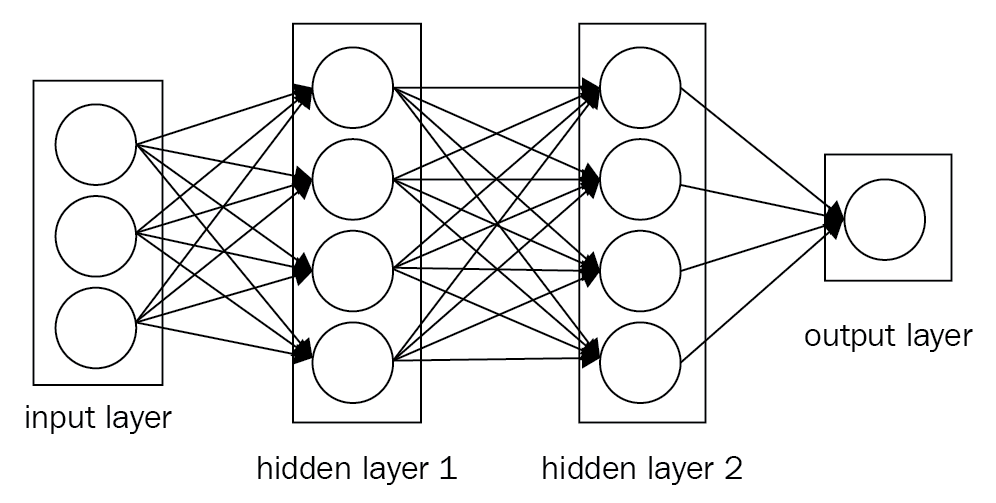
\includegraphics[width=\imgMed]{images/theory/neural_network.png}
    \caption{Ein \textit{fully-connected ANN} mit zwei versteckten Schichten \cite{Sewak2018}}
    \label{fig:ful_con_ann}
\end{figure}

Um nun genauer nachzuvollziehen, wie ein Knoten in einem ANN operiert, gehen wir genauer auf die mathematische Definition eines Knotens ein. \\
Die Verarbeitung der Eingabevektoren erfolgt durch die Anwendung der sogenannten Aktivierungsfunktion $a$. Die Aktivierungsfunktion ist die Summe der gesamten Eingabevektoren $[x_1,…,x_n]$ multipliziert mit einer Gewichtsmatrix $[w_1,...,w_n]^T$,
wobei \textit{n} die Anzahl der vorherigen Knoten ist. Mathematisch ist sie wie folgt definiert:

\[a = \sum_{i=1}^{n} x_i w_i\]

In der Abbildung \ref{fig:act_fun} wird die Aktivierungsfunktion $a$ dargestellt. Es ist erkennbar, wie jeder Eingabevektor $x_i$ mit einem Gewicht $w_i$ multipliziert wird und anschließend die Summe aller Ergebnisse gebildet wird. Das Ergebnis der Aktivierungsfunktion $a$ ist die Ausgabe eines Knotens und wird anschließend von den folgenden Knoten in der nächsten Schicht als Eingabevektor verarbeitet.

\begin{figure}[H]
    \centering
    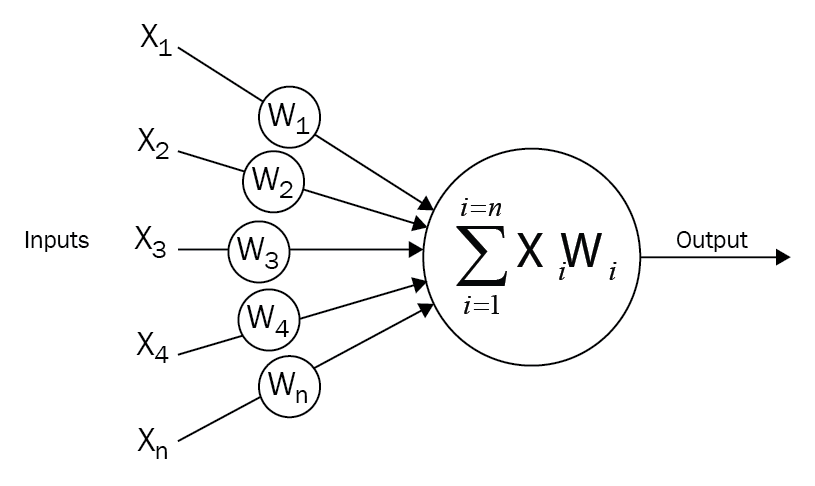
\includegraphics[width=\imgMed]{images/theory/activationfunction.png}
    \caption{Bildliche Darstellung der \textit{Aktivierungsfunktion} \cite{Sewak2018}}
    \label{fig:act_fun}
\end{figure}

Mit dieser Funktion können wir nachvollziehen, wie jeder einzelne Knoten seine Entscheidung trifft.\cite*{Braspenning1995}

Zusätzlich können wir eine \textit{Verlustfunktion} für das Netzwerk definieren, um die Genauigkeit der Entscheidungen zu messen. Bei den ANN existieren zwei verschiedene Arten von Verlustfunktionen, die Klassifizierungs-Verlustfunktion und die Regression-Verlustfunktion.
Die Klassifizierung-Verlustfunktion wird genutzt, wenn ein Netzwerk als Klassifizierer eingesetzt wird, wie es in diesem Test der Fall ist. Die Regression-Verlustfunktion wird bei Anwendungen der Vorhersage von bestimmten Werten verwendet.
Unter den zwei Arten der Verlustfunktion für ANN existieren wiederum verschiedene mathematische Funktionen, mit denen sich der Wert je nach Anwendung berechnen lässt.\cite{dwivedi_2020}

Im Folgenden wird die sogenannte \textit{Kreuzentropie} oder auch \textit{log-loss} genannt als Verlustfunktion verwendet. Diese Verlustfunktion wird bei binärer Klassifikation eingesetzt und berechnet den Verlustwert mit Hilfe eines booleschen Wertes und dem errechneten Entscheidungswert des ANN. Der boolesche Wert wird durch 0 oder 1 ausgedrückt, dieser sagt aus, ob das zu klassifizierende Objekt richtig erkannt wurde oder nicht. In der Abbildung \ref*{fig:crossentropy} wird die Kreuzentropie dargestellt. Anhand dieser Darstellung ist zu erkennen, wie der Verlustwert abhängig vom Entscheidungswert des ANN ist. Wenn der Entscheidungswert sich der 1 annähert, verringert sich der Wert der Kreuzentropie.
Für eine Klassifikation von zwei Klassen wird die Kreuzentropie wie folgt berechnet:

\[-(y\times log(p) + (1 - y) \times log(1-p))\]

\begin{itemize}
    \item $y$ ist der boolesche Wert, der angibt, ob das zu klassifizierende Objekt richtig erkannt wurde.
    \item $p$ ist der errechnete Entscheidungswert des ANN.
\end{itemize}

Im Fall der Zahlenerkennung existiert für jede Zahl eine Klasse. Das Prinzip der Kreuzentropie lässt sich auf eine beliebige Anzahl von Klassen erweitern, in dem für jedes Label pro Beobachtung der Verlustwert berechnet wird und letztendlich summiert wird.

\[ -\sum_{c=1}^{M}y_{o,c} \times log(p_{o,c}) \]

\begin{itemize}
    \item $c$ ist das Klassenlabel.
\end{itemize}
\cite{10.2307/2348828}

\begin{figure}[H]
    \centering
    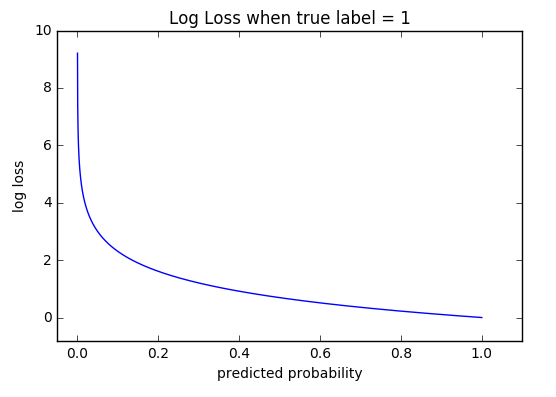
\includegraphics[width=\imgMed]{images/theory/cross_entropy.png}
    \caption{Graph einer \textit{Kreuzentropie} \cite{fortuna_viana_2019}}
    \label{fig:crossentropy}
\end{figure}

\subsubsection*{Von Artificial Neural Network zu Convolutional Neural Network}
Wie im Vorfeld angeführt, handelt es sich bei den CNN um eine Spezialisierung eines ANN. Diese Spezialisierung erweitert und spezifiziert Aspekte eines ANNs, welche im Folgenden genauer erläutert werden.

Da wir das CNN für die Klassifikation von Bildinhalten verwenden, muss die Eingabeschicht für diesen Datentypen vorbereitet werden. Die Besonderheit hierbei liegt darin, dass die Knoten zusätzlich zu den Schichten in drei Dimensionen aufgeteilt werden. Diese Aufteilung bezieht sich jedoch nur auf die Verknüpfungen zu den Knoten in der nächsten Schicht. Die Dimensionen sind für ein Bild die Höhe und Breite. Eine zusätzliche dritte Dimension ist die sogenannte Tiefe, welche Auskunft über die Anzahl der folgenden verknüpften Knoten bietet.

Die Architektur der CNN erweitert das Prinzip der Ein/Ausgabeschicht und den versteckten Schichten insoweit, als dass die versteckten Schichten in weitere Kategorien eingeteilt werden können. Bei einem CNN gibt es zusätzlich zu der Ein/Ausgabeschicht, die Filter-Schichten (engl. Convolutional Layer), Aggregations-Schichten (Pooling Layer) und die vollständig verbundenen Schichten (engl. Fully Connected Layer, Dense Layer).
Bei der Ausgabeschicht handelt es sich ebenfalls um eine vollständig verbundene Schicht. \cite*{Keiron2015}

Die einzelnen Aufgaben und Eigenarten der verschiedenen Schichten werden im Folgenden behandelt.

\subsubsection{Input Layer}
In der Eingabeschicht werden die Bilddaten gespeichert und in einer dreidimensionalen Matrix dargestellt.\cite*{Sewak2018}

\subsubsection{Filter-Schicht}
Die Filter-Schicht, auch häufig als Feature-Extraction-Layer bezeichnet, extrahiert Eigenschaften aus dem Eingabebild und übt die Hauptanzahl an Berechnungen aus.
Es handelt sich hierbei um Faltungsoperationen, die Ähnlichkeiten zur Fourier-Transformation und zur Lapace-Transformation aufweisen, und bilden das Merkmal eines CNNs.
Ein Neuron einer Filter-Schicht betrachtet einen bestimmten Bereich einer vorherigen Schicht in Form einer Matrix und bildet daraus ein Skalarprodukt, um die den Bereich auf nur eine Zahl zu reduzieren.
Die Architektur eines CNNs, die aus den verschiedenen Schichten und der Filter-Schichten besteht, ermöglichen, dass weniger Neuronen benötigt werden im Gegensatz zu anderen vielschichtigen neuronalen Netzwerken.\cite*{Sewak2018}
Die Knoten in der Filter-Schicht nutzen die sogenannte \ac{ReLU}-Funktion als Aktivierungsfunktion. Diese ist, wie der Name bereits beschreibt, eine lineare Funktion, welche leicht modifiziert ist, sodass der Rückgabewert der Funktion gleich null ist, wenn der Eingabewert kleiner gleich null ist. Das bringt diverse Vorteile bei der Optimierung von CNNs und ANNs. Lineare Funktionen sind leichter zu optimieren und zu trainieren. Die ReLU Funktion lässt sich mathematisch als das Maximum einer Menge definieren, welche zwei Elemente besitzt, den Wert $0$ und den Wert $x$.

\[ReLU(x) = max\{0, x\}\] \cite*{goodfellow2016}

\subsubsection{Aggregations-Schicht}
Die Aggregations-Schicht ist für das Heruntertasten der Dimensionen zuständig, um die Parameter der Aktivierungsfunktion zu reduzieren. Durch die Anwendung der zuvor liegenden Filter-Schichten wird die räumlichen Dimension erhöht und die damit einhergehend Anzahl der Parameter der darauf folgenden Schicht. Dies hat zur Folge, dass die Komplexität des Models erhöht wird. Diese Überanpassung wird mit den Aggregations-Schichten entgegengewirkt.\cite*{Sewak2018}
Für das Skalieren wird am häufigsten die \textit{max pooling} Funktion verwendet. Diese Funktion reduziert die Dimensionen, ausgenommen der Tiefe, auf eine Größe von etwa 25\% der Originalgröße.\cite*{Keiron2015}

\subsubsection{Vollständig-Verbundene-Schicht}

Die vollständig verbundene Schicht ist die einer versteckten Schicht in einem ANN gleich. Diese Schicht ist hauptsächlich für die Klassifizierung und Berechnungen der Wahrscheinlichkeit zuständig. Die Aktivierungsfunktion der Knoten in dieser Schicht ist wie bei der Filter-Schichten die ReLU Funktion.
Einleitet wurde erwähnt, dass es sich bei der Ausgabeschicht ebenfalls um eine vollständig verbundene Schicht handelt. Diese wird auch als \textit{soft-max} Schicht bezeichnet und gibt die letztendliche Klassifizierung des Bildes zurück.\cite*{Sewak2018}

\newpage

\subsubsection{Bewertung ded Convolutional Neural Networks}

Damit wir ein CNN mit der SVM und dem KNN vergleichen können, werden dieselben Bewertungskriterien untersucht. Die für die Bewertung relevanten Kriterien waren:

\begin{itemize}
    \item Komplexität
    \item Genauigkeit
    \item Präzision
    \item Einfachheit der Umsetzung
\end{itemize}

Bevor wir genauer auf die Bewertungskriterien eingehen, werden wir uns mit dem für den Test konstruierten CNN beschäftigen.
Dieser wurde in der Programmiersprache \textbf{Python} Version 3.9 geschrieben. Für die Konstruktion und die Ausführung des Tests benötigen wir verschiedene Bibliotheken, die dabei helfen können, die Bewertungskriterien zu ermitteln, sowie den CNN zu modellieren. Bei diesem Test wurde die Bibliothek \textbf{Tensorflow} verwendet, welche wiederum die \textbf{Keras} Bibliothek verwendet. Zusätzlich wurde die Bibliothek \textbf{NumPy} und \textbf{matplotlib} verwendet, um mit Hilfe von \textit{NumPy} die Daten zu strukturieren und mit \textit{matplotlib} die Ergebnisse darzustellen. Den Programmcode zum Importieren der notwendigen Bibliotheken, sowie die Vorbereitung für den CNN ist in Codeabschnitt \ref{lst:test_prep_cnn} zu finden. In diesem Abschnitt werden zunächst die Bibliotheken importiert und die MNIST-Datenbank wird geladen. Beim Laden der Daten werden die Daten bereits in Trainingsobjekte und Testobjekte unterteilt.

\begin{minipage}{\textwidth}
    \begin{lstlisting}[language=Python, caption=Pythoncode zur Testvorbereitung vom CNN, label=lst:test_prep_cnn]
import tensorflow as tf
import numpy as np
import matplotlib.pyplot as plt
from keras import backend as K

mnist = tf.keras.datasets.mnist

(x_train, y_train), (x_test, y_test) = mnist.load_data()

y_train = y_train.astype('float32')
y_test = y_test.astype('float32')

# Erstellung von Binaerendaten 
mask = x_train > 127.5
maskb = x_train <= 127.5
x_train[mask] = 255
x_train[maskb] = 0

# Shift to -1 to 1
x_train, x_test = (x_train - 127.5) / 127.5, (x_test - 127.5) / 127.5

# Datenaufteilung fuer Validierung
x_val = x_train[-10000:]
y_val = y_train[-10000:]
x_train = x_train[:-10000]
y_train = y_train[:-10000]

	\end{lstlisting}
\end{minipage}

Im folgenden Codeabschnitt wird das CNN-Model definiert. Das Model wurde mit folgenden Schichten definiert:

\begin{itemize}
    \item Filter-Schicht (Eingabeschicht)
    \item Filter-Schicht
    \item Filter-Schicht
    \item Aggregations-Schicht
    \item Vollständig-verbundene-Schicht
    \item Vollständig-verbundene-Schicht (Ausgabeschicht)
\end{itemize}

Die zusätzlich zu sehenden Schichten \textit{Dropout} und \textit{Flatten} wurden definiert, um die Komplexität des Models zu reduzieren. Dieser Effekt ist nur während des Trainierens sichtbar. Bei der \textit{Dropout}-Schicht handelt es sich um eine Schicht, die mit einer gewählten Wahrscheinlichkeit von \textit{0,25} einen Knoten aus der Schicht ausschaltet, um \textit{overfitting} zu verhindern. Die \textit{Flatten}-Schicht formt die mehrdimensionalen Daten in eine einzelne Dimension um, damit diese von der vollständig-verbunden-Schicht verarbeitet werden kann.

\begin{minipage}{\textwidth}
    \begin{lstlisting}[language=Python, caption=Pythoncode zur Konstuktion vom CNN, label=lst:test_cnn]
#CNN
model = tf.keras.models.Sequential([
		tf.keras.layers.Conv2D(32, kernel_size=(3, 3),
							activation='relu',
							input_shape=(28, 28, 1)),
	tf.keras.layers.Conv2D(32, kernel_size=(3, 3),
							activation='relu'),
	tf.keras.layers.Conv2D(32, kernel_size=(3, 3),
							activation='relu'),
	tf.keras.layers.MaxPooling2D(pool_size=(2, 2)),
	tf.keras.layers.Dropout(0.5),
	tf.keras.layers.Flatten(),
	tf.keras.layers.Dense(128, activation='relu'),
	tf.keras.layers.Dropout(0.25),
	tf.keras.layers.Dense(10, activation='softmax')
])

model.summary()
model.compile(optimizer='adam',
              loss='sparse_categorical_crossentropy',
              metrics=['accuracy', precision_m])

x_train = np.reshape(x_train, (x_train.shape[0], x_train.shape[1], x_train.shape[2], 1))
x_test = np.reshape(x_test, (x_test.shape[0], x_test.shape[1], x_test.shape[2], 1))
x_val = np.reshape(x_val, (x_val.shape[0], x_val.shape[1], x_val.shape[2], 1))
				
model_data = model.fit(x_train, y_train, epochs=10, batch_size=128, validation_data=(x_val, y_val))
model.evaluate(x_test, y_test, verbose=2)
\end{lstlisting}
\end{minipage}

\begin{minipage}{\textwidth}
    \begin{lstlisting}[language=Python, caption=Pythoncode zum Darstellen der Daten, label=lst:test_plot_cnn]
print(model_data.history)
plt.subplot(2, 1, 1)
plt.plot(model_data.history['accuracy'])
plt.plot(model_data.history['val_accuracy'])
plt.title('model accuracy')
plt.ylabel('accuracy')
plt.xlabel('epoch')
plt.legend(['train acc', 'val acc'], loc='lower right')
plt.subplot(2, 1, 2)
plt.plot(model_data.history['precision_m'])
plt.plot(model_data.history['val_precision_m'])
plt.title('model precision')
plt.ylabel('precision')
plt.xlabel('epoch')
plt.legend(['train precision', 'val precision'], loc='upper right')
plt.tight_layout()
plt.show()
	\end{lstlisting}
\end{minipage}

\subsubsection{Komplexität}
Die \textit{Zeit}-Komplexität von einem CNN-Modell ist die Summe der \textit{Zeit}-Komplexitäten der einzelnen Schichten. Die genaue Berechnung als auch die genaue \textit{Zeit}-Komplexität des oben erstellten Modells übertrifft den Rahmen dieser Arbeit. Für einen ausreichenden Vergleich zwischen den vorgestellten Klassifizierern wird lediglich die Komplexität der Filter-Schicht betrachtet. Die O-Notation der Filter-Schicht lautet wie folgt:

\[\sum^{d}_{l=1}n_{l-1} * s^2_l * n_l * m^2_l \]

\begin{itemize}
    \item $l$ ist der Index von einer Filter-Schicht
    \item $d$ ist die Anzahl der Filter-Schichten in einem Netzwerk
    \item $n_l$ ist die Anzahl der Knoten in der $l$-ten Filter-Schicht
    \item $n_{l-1}$ ist die Anzahl der Eingabeparameter
    \item $s_l$ ist die dritte Dimension der Filter-Schicht
    \item $m_l$ ist die Anzahl der Features die in der $l$-ten Filter-Schicht ausgegeben werden
\end{itemize}
\cite{Kaiming_2014}

\subsubsection{Genauigkeit \& Präzision}

Um die Präzision vom CNN zu berechnen, muss zuerst eine Hilfsfunktion definiert werden, damit dieser Wert verfolgt wird. Die Metrik der Präzision wurde aus der Keras-Bibliothek 2.0 entfernt. Eine Lösung des Problems hat der Benutzer \textit{Tasos} auf \textit{StackExchange} veröffentlicht. \cite{stackexchange_2020}

\begin{minipage}{\textwidth}
    \begin{lstlisting}[language=Python, caption=Hilfsfunktion für Präzision \cite{stackexchange_2020}, label=lst:func_precision]
def precision_m(y_true, y_pred):
	true_positives = K.sum(K.round(K.clip(y_true * y_pred, 0, 1)))
	predicted_positives = K.sum(K.round(K.clip(y_pred, 0, 1)))
	precision = true_positives / (predicted_positives + K.epsilon())
	return precision	
	\end{lstlisting}
\end{minipage}


Die Genauigkeit und die Präzision des CNN-Modells kann aus den Ausgaben der Epochenmetriken gelesen werden. Das Ergebnis der letzten Epoche wird in \ref{lst:test_cnn_results} dargestellt. Es ist zusehen, dass das CNN-Modell eine Genauigkeit von \textbf{99\%} und eine Präzision von \textbf{92\%} erreicht.

\begin{minipage}{\textwidth}
    \begin{lstlisting}[language=Bash, caption=Testergebnisse vom CNN, label=lst:test_cnn_results]
...
Epoch 10/10
391/391 [==============================] - 76s 195ms/step - loss: 0.0273 - accuracy: 0.9909 - precision_m: 0.9264 - val_loss: 0.0374 - val_accuracy: 0.9891 - val_precision_m: 0.9191
313/313 - 2s - loss: 0.0253 - accuracy: 0.9916 - precision_m: 0.9209 - 2s/epoch - 5ms/step
	\end{lstlisting}
\end{minipage}

\subsubsection{Einfachheit der Umsetzung}
In der Bewertung von diesem Kriterium wird von einem subjektiven Standpunkt ausgegangen. Es soll bewertet werden, wie einfach die Umsetzung des CNN-Modells in diesem Projekt ist.
Das CNN-Modell wird mit \textbf{3/5} Punkten bewertet.
Auch wenn das Forschungsgebiet der CNN in Bezug der Handschrifterkennung sehr gut beleuchtet ist, ist vor allem die Optimierung und Umsetzung eines CNNs komplex.
Der CNN wird, ähnlich wie die anderen Algorithmen, bereits durch eine Bibliothek bereitgestellt, aber die Funktionen benötigen viele Parameter, wie zum Beispiel die Anordnung und die Definition der verschiedenen Schichten.
\newpage
